\documentclass[main]{subfiles}
\begin{document}

%@@@@@@@@@@@@@@@@@@@@@@@@@@@@@@
\noindent
\textbf{Topics: Feed-Forward Networks and Backpropagation - 05.12.2019} \\
Lecturer: Dr. Matthew Cook \\
Author: Vanessa Leite \{vanessa at ini.uzh.ch\}

\section{Feed-Forward Networks}

In the Feed-forward networks, the information moves in only one direction (forward) from the input nodes, through the hidden nodes (if they exist), and to the output nodes.
\textbf{There are no cycles in this network.}
\begin{itemize}[noitemsep,nolistsep]
	\item Multiple layers of neurons with a certain number of inputs and outputs.
	\item Every laxer of nodes feeds the next layer with inputs.
	\item There is an input and an output layer with hidden layers in between.
\end{itemize}

\begin{figure}[H]
	\centering
	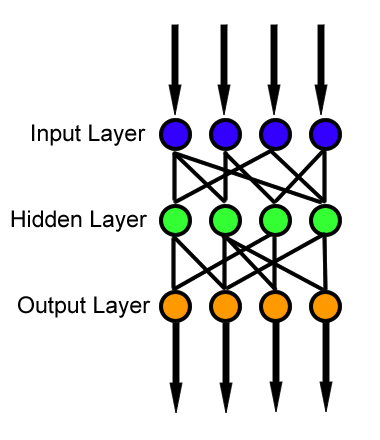
\includegraphics[width=0.25\textwidth]{Feed_forward_neural_net.png}
\end{figure}

A single unit, like a perceptron, can be seen as a feed-forward network.

\subsection{Boltzmann Machines}

\subsection{Backpropagation and Error function}
\begin{itemize}[noitemsep,nolistsep]
	\item The inputs and desired outputs are given as $S=\{(x,d)^1,\ldots,(x,d)^l\}$.
	\item The error function is given as $E(S) = \sum_i\frac{1}{2}||y(x^i)-d^i||^2$.
	\item The output is a non-linear transformation $y=f(a)$.
	\item $f(a)$ is the activation function, which is usually a sigmoid function.
	\item The error function for a single training sample is $E(S)=\frac{1}{2}(f(x_1w_1+x_2w_2+w_0)-d)^2$.
	\item The output of a simple network is for example $y(x_1,x_2,x_3)=f(x_1w_{21}+f(x_2w_{11}+x_3w_{12}+w_{10})w_{22}+w_{20})$.
	\item $\frac{\partial E(w_1,w_2,w_0)}{\partial w_1}=(f(x_1w_1+x_2w_2+w_0)-d)\cdot f'(x_1w_1+x_2w_2+w_0)\cdot x_1$.
	\item $\frac{\partial E(w_1,w_2,w_0)}{\partial w_2}=(f(x_1w_1+x_2w_2+w_0)-d)\cdot f'(x_1w_1+x_2w_2+w_0)\cdot x_2$.
	\item $\frac{\partial E(w_1,w_2,w_0)}{\partial w_0}=(f(x_1w_1+x_2w_2+w_0)-d)\cdot f'(x_1w_1+x_2w_2+w_0)$.
	\item The error terms travel backwards through the network and get multiplied with the derivative of the activation function of that input. Multiple error terms can just be added up.
	\item The partial derivative of the error $E$ term in relation to the weight $w$ to be adjusted can be added to the weight in order to learn. An additional weighting factor can be added.
\end{itemize}

\subsection{Gradient Descent}
Consider $E = \sum(f_w(x) - y_i)^2$, we want to adjust $\vec{w}$ (weights of the network) to minimize $E$.

$\frac{dE}{df} = \sum 2(f_{\vec{w}} (x) - y_i)$.

\begin{figure}[H]
	\centering
	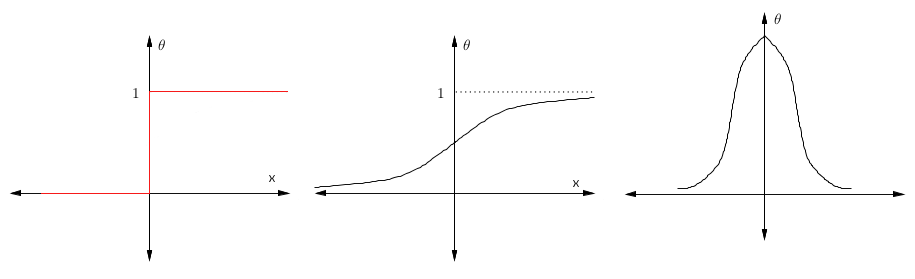
\includegraphics[width=0.6\textwidth]{activation-functions.png}
	\caption{left-most figure: $f_{w_0} (x) = \theta(wf + w...)$, $\frac{df}{dw} = 0 \rightarrow \theta$ is not a good threshold function. Using a new threshold function (center figure). Right figure: $\frac{df}{dw} = \theta\prime$.}
\end{figure}

\end{document}
